\documentclass[12pt,a4paper]{article}
\usepackage[utf8]{inputenc}
\usepackage[spanish]{babel}
%\usepackage{amsmath}
%\usepackage{amsfonts}
%\usepackage{amssymb}
\usepackage{hyperref}
\usepackage[pdftex]{graphicx}
\usepackage{fancyhdr}
\usepackage[font=small,labelfont=bf]{caption}
\pagestyle{fancy}
\lhead{\bfseries Redes de Datos -- Cloud Computing}
\rhead{}
%\chead{}
\newcommand{\HRule}{\rule{\linewidth}{0.5mm}}
\usepackage[left=2cm,right=2cm,top=2cm,bottom=2cm]{geometry}
\author{Ignacio Perez Laborda}

\hypersetup{pdfborder = {0 0 0}}

\begin{document}

\begin{titlepage}

\begin{center}

% Upper part of the page

\includegraphics[width=0.25\textwidth]{./logo_UB.png}\\[1cm] 

\textsc{\LARGE Universidad de Belgrano}\\[1.5cm]

\textsc{\Large Redes De Datos}\\[0.5cm]

%title
\HRule \\[0.4cm]
{ \huge \bfseries Trabajo Practico 2 -- Cloud Computing}\\[0.4cm]
\HRule \\[1.5cm]

% Author and supervisor
\begin{minipage}{0.4\textwidth}
\begin{flushleft} \large
\emph{Alumno:}\\
Ignacio \textsc{P\'erez Laborda}\\
Barbara \textsc{Mart\'inez}\\
\end{flushleft}
\end{minipage}
\begin{minipage}{0.4\textwidth}
\begin{flushright} \large
\emph{Matricula:} \\
502--10426\\
502--10402\\
\end{flushright}
\end{minipage}\\[1.5cm]

\vfill

%Bottom of the page
{\large \today}

\end{center}

\end{titlepage}


\tableofcontents

\listoffigures

\newpage

\section{¿Que es Cloud Computing?}

\subsection{Introducción}
Cuando se trata de un desarrollo, un problema muy común es la
infraestructura. Las grandes empresas tienen el capital
suficiente como para contratar a un ingeniero capaz de diseñar
una red de infraestructura adecuada a la información que se
maneja y a un personal que se encargue de administrar esa
red. Pero ¿Qué pasa cuando gente emprendedora que quiere empezar
un proyecto no tiene que almacenar la información suficiente
como para aprovechar, o no puede costear, un salón de
servidores? ¿O cuando se crea una aplicación que tiene un uso
temporal? ¿O se lanza una aplicación la cual no se sabe si
tendrá el suficiente éxito como para gastar fortunas en
infraestructura?. La respuesta es Cloud Computing, concepto
conocido también bajo los términos servicios en la nube. Es un
servicio de almacenamiento en el cual cualquier usuario puede
acceder a el sin las complicaciones que lleva montar
servidores, diseñar una topología y adecuar un ambiente para su
correcto desempeño. El usuario final no necesita tener
conocimientos avanzados de informática para utilizar estos
servicios ya que se puede presentar de muchas formas de cloud
computing, y quizás ni siquiera lo notemos, desde almacenamiento
de archivos que usamos cotidianamente y queremos tenerlos al
alcance siempre, hasta soporte de almacenamiento de datos para
aplicativos de proyectos caseros. Su versatilidad hace que hasta
también se adecúe al equipo y al tipo de plataforma en el cual
nos estemos conectando para visualizar nuestra información,
tablets, equipos de escritorio, celulares, entre otros.\par

La computación en la nube son servidores desde internet
encargados de atender las peticiones en cualquier momento. Se
puede tener acceso a su información o servicio, mediante una
conexión a internet desde cualquier dispositivo móvil o fijo
ubicado en cualquier lugar. Sirven a sus usuarios desde varios
proveedores de alojamiento repartidos frecuentemente por todo el
mundo. Esta medida reduce los costes, garantiza un mejor tiempo
de actividad y que los sitios web sean invulnerables. Es un nuevo
modelo de prestaciones que hasta le permite al usuario tener un
catálogo online de todos los servicios que ofrece, aumentando
mas una de sus cualidades mas importantes que es la
flexibilidad. Esto genera beneficios tanto para los proveedores,
que pueden ofrecer, de forma más rápida y eficiente, un mayor
número de servicios, como para los usuarios que tienen la
posibilidad de acceder a ellos, disfrutando de la
``transparencia'' e inmediatez del sistema y de un modelo de pago
por consumo, así el consumidor puede controlar sus gastos.\par 
Se incorporan conceptos como  el ``software como servicio'' y otros
mas recientes que son tendencias tecnológicas que tienen en
común el que confían en Internet para satisfacer las necesidades
de cómputo de los usuarios.


\begin{figure}[h!]
 \centering
 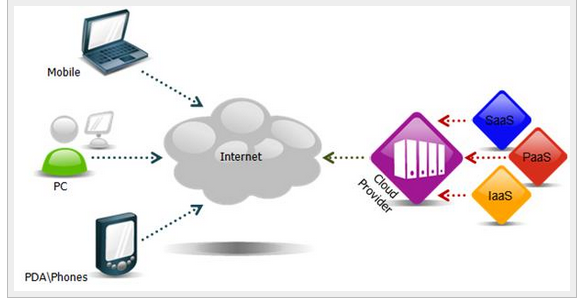
\includegraphics[width=0.71\textwidth]{cc_def.png}
\caption[Ruta de datos]{Ruta de la información en cloud
computing}
\end{figure}

\par
\subsection{Características importantes de Cloud Computing}

Para obtener la eficiencia que se conoce hoy en día, cloud
computing atiende a una serie de características básicas que las
difieren de otros servicios de almacenamiento:
\begin {itemize}
\item \textbf{Flexibilidad en la elección de aplicaciones:} El
usuario puede decidir en todo momento qué aplicaciones usar y
elegir entre aquellas que son gratuitas y las que no lo son. En
el caso de las aplicaciones de pago, el coste irá en función de
diversas variables, como el servicio contratado, el tiempo que
se ha usado ese servicio, el volumen de tráfico de datos
utilizado, etc.
\item \textbf{Accesibilidad:} Se encuentra una disponibilidad
completa de las aplicaciones en cloud computing y libres para el
usuario. El rango es muy amplio y varía desde el uso de PCs hasta
portátiles y móviles.

\item \textbf{Asignación de recursos en modo multiusuario:} A
diferencia de las aplicaciones de software tradicionales, en el
cloud computing el proveedor tiene una única aplicación que abre
a todos los usuarios que desean utilizarla, estableciendo unos
recursos de acceso y prestaciones distintos para cada usuario.
Al ser aplicaciones multiusuario, puede hacer miles de
internautas utilizando la misma herramienta a la vez, cada uno
con las mismas o distintas prestaciones.

\item \textbf{Elasticidad y escalabilidad:} Las aplicaciones en
cloud son totalmente elásticas en cuanto a su rapidez de
implementación y adaptabilidad. Además, son totalmente
escalables, es decir, hoy podemos estar utilizando solo un 10
\% del total de la aplicación y mañana podemos acceder al 80
\% de la misma con total normalidad y rapidez, con tan solo
comunicarlo a nuestro proveedor y modificar nuestra tarifa de
suscripción.
 
\item \textbf{Supervisión del servicio:} Los sistemas en cloud
controlan y optimizan el uso de los recursos de manera
automática, por lo que el uso de estos puede seguirse,
controlarse y notificarse, lo que aporta transparencia tanto
para el proveedor como para el consumidor del servicio
utilizado.
 
\item \textbf{Seguridad:} Los datos, cuando están en aplicaciones
en cloud, se alojan en DATA CENTERS, empresas específicamente
dedicadas a la custodia y salvaguarda de datos de empresas de
todo tipo. Son empresas que cuentan con todas las medidas de
seguridad necesarias, tanto físicas como de software, de forma
que no haya jamás una pérdida de información ni de integridad de
los datos.
\end{itemize}

\begin{figure}[h!]
 \centering
 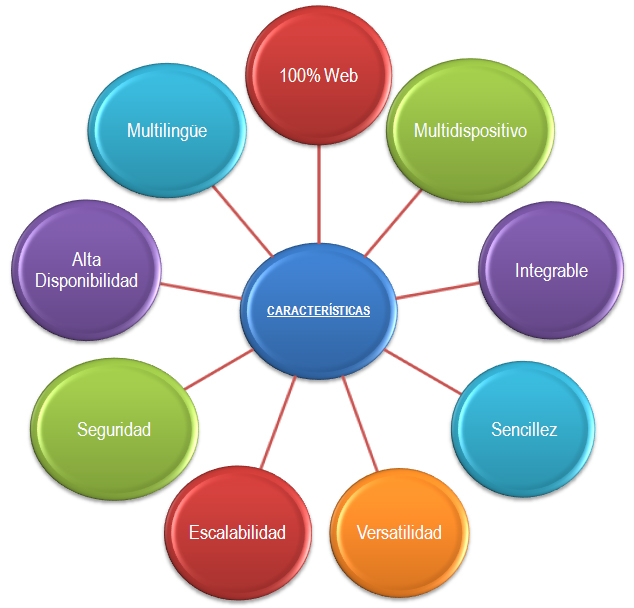
\includegraphics[width=0.61\textwidth]{Caracteristicas2.png}
 \caption[Características]{Características del cloud computing}
\end{figure} 

\subsection{Las Ventajas de Cloud Computing}

\begin {itemize}
\item \textbf{Mejora en la economía} El poder aumentar la
capacidad de producción con la menor cantidad de
personas. Asegura un mayor rendimiento costo-beneficio.

\item \textbf{Reducir el gasto en infraestructura tecnológica}
Se otorga un fácil acceso a la información con un gasto fijo y
mínimo por adelantado.

\item \textbf{Globalización de la fuerza de trabajo} Todas las
personas pueden acceder a la nube siempre y cuando tengan
conexión a internet.
\item \textbf{Optimización de los procesos} Hacer mayor trabajo
en menos tiempo.
 
\item \textbf{Reducir los costos de capital} No hay necesidad de
gastar dinero en hardware, software o licencias.
 
\item \textbf{Mejora la accesibilidad} Acceso en cualquier
momento y en cualquier lugar.
  
\item \textbf{Supervisar los proyectos con mayor eficacia}
Facilidad para supervisar el tiempo y costo de los proyectos y
presupuestarlos.
 
\item \textbf{ Menos entrenamiento de personal} No hay que
gastar recursos en capacitación de personal ya que solo se
requieren conocimientos mínimos de software.
  
\item \textbf{ Mejorar la flexibilidad} Puede cambiar de
capacidad fácilmente y adaptarlo rápidamente a las necesidades
del usuario.
    
\end{itemize}


\begin{figure}[h!]
 \centering
 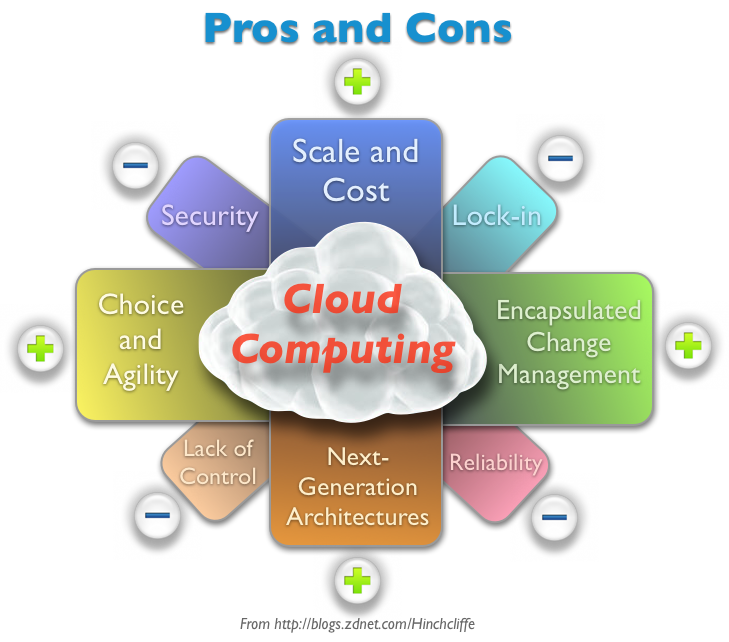
\includegraphics[width=0.54\textwidth]{cc_pros.png}
\caption[Pros Cloud Computing]{Esquema de ventajas y desventajas de cloud computing}
\end{figure}\par


\section{Distintos Servicios de Cloud Computing}
\subsection{SaaS -- Software as a Service}
En el sistema tradicional un cliente compra o manda a hacer una aplicación y 
este es dueño de una licencia, se le entrega físicamente el código fuente o
el binario listo a ser ejecutado de esa manera por cada instancia del 
programa hacia falta tener una licencia. Además la disponibilidad de los 
programas y la instalación corrían a cargo del cliente implicando mayores 
gastos. También muchas veces se pagaba por un software no muy adaptado a las 
necesidades especificas sino a términos mas generales, la personalizacion del 
software se volvía muy cara y dificultosa.\par
Saas es aquella aplicación ofrecida por su creador (ISV) a través de internet 
para su uso o utilización por varios clientes manteniendo la privacidad de 
sus datos y la personalización de la aplicación. El usuario paga por el uso, 
por la infraestructura necesaria (CPD, máquinas de computación, de 
almacenamiento, de seguridad,etc) para el correcto funcionamiento de la 
aplicación y por el mantenimiento (nuevas versiones, corrección de bugs, 
almacenamiento necesario,etc) de la infraestructura y aplicación.\par
El hecho de que se acceda a la aplicación a través de internet no quiere 
decir que se haga a través de navegador pero la utilidad más interesante de 
este tipo de aplicaciones es que se haga a través del navegador y no requiera 
instalación en las máquinas de los usuarios de la aplicación. En esta 
comparativa entre saas y el software instalado in-house  podemos sacar 
conclusiones de los beneficios del saas.\par
El modelo Saas establece estas características:
\begin{itemize}

\item \textbf{Configuración y customizacion: }
Las aplicaciones Saas soportan lo que tradicionalmente se conoce como 
personalizacion de aplicaciones. En este caso un cliente puede alterar un 
conjunto de parámetros de configuración que afectan el look and feel y cierta 
funcionalidad. De esta manera cada cliente puede tener su propia 
configuración.

\item \textbf{Accelerated feature delivery}
Las aplicaciones Saas son actualizadas frecuentemente. Esto se logra por el 
hecho de que la aplicación se encuentra hosteada en un solo lugar y la 
actualización es decidía por el proveedor no los clientes.Esto se ve 
acentuado por las metodologías agiles las cuales permiten lanzamientos en 
menor tiempo. 

\item \textbf{Uso de protocolos abiertos}
Dados que estos sistemas no acceden a las compañías y no necesariamente 
interactúan con otros sistemas se aseguran de operar con estándares abiertos
de esta manera se pueden interconectar con una mayor cantidad de clientes y 
ofrecer el servicio a mas mercados.

\end{itemize}

Las ventajas son:
\begin{enumerate}

\item No es necesario que el cliente cuente con un área especializada de 
soporte para el sistema, por lo que se reducen sus costes y riesgo de 
inversión.
\item La responsabilidad de la operación recae en la empresa IT. Esto 
significa que la garantía de disponibilidad de la aplicación y su correcta 
funcionalidad, es parte del servicio que da la compañía proveedora del 
software.
\item La empresa IT no desatiende al cliente. El servicio y atención continua 
del proveedor al cliente es necesaria para que este último siga pagando el 
servicio.
\item La empresa IT provee los medios seguros de acceso en los entornos de la 
aplicación. Si una empresa IT quiere dar SaaS en su cartera de productos, 
debe ofrecer accesos seguros para que no se infiltren datos privados en la 
red pública.
\item No es necesaria la compra de una licencia para utilizar el software, 
sino el pago de un alquiler o renta por el uso del software. Aunque también 
se dan casos particulares donde el servicio es totalmente gratuito, como por 
ejemplo en el servicio de blogs que brindan diferentes compañías: Wordpress, 
Blogger, etc; es decir, se cuenta con el servicio, se puede acceder 
libremente, se garantiza usabilidad y actualidad, pero no se paga por el 
servicio.
\item Se le permite al cliente completa flexibilidad en el uso de los 
sistemas operativos de su preferencia, o al cual pueda tener acceso.

\end{enumerate}

Mientras que las desventajas son:
\begin{enumerate}

\item La persona usuaria no tiene acceso directo a sus contenidos, ya que 
están guardados en un lugar remoto, y en caso de no contar con mecanismos de 
cifrado y control disminuye el índice de privacidad, control y seguridad que 
ello supone, ya que la compañía TI podría consultarlos.
\item El usuario no tiene acceso al programa, por lo cual no puede hacer 
modificaciones (dependiendo de la modalidad del contrato de servicios que 
tenga con la compañía TI).
\item Al estar el servicio y el programa dependientes de la misma empresa, no 
permite al usuario migrar a otro servicio utilizando el mismo programa 
(dependiendo de la modalidad del contrato de servicios con la compañía de 
TI).
\item Si el servicio de Internet no está disponible por parte del ISP, el 
usuario no tendrá acceso al programa, por lo que sus operaciones se verán 
afectadas hasta que dicho servicio se restablezca.

\end{enumerate}

\subsubsection{Ejemplo de prestadoras de servicio}

\subsection{PaaS -- Platform as a service}
\subsection{IaaS -- Infrastructure as a service}

\section{Aplicaciones Practicas}

\section{Cloud Computing para usuarios finales}

\section{Conclusiones}

\newpage

\begin{thebibliography}{1}

\bibitem{caractCC}		
\emph{Caracteristicas de las aplicaciones. }
 21 Abr 2013\\
\url{http://www.societic.com/2010/03/cloud-computing-caracteristicas-de-las-
aplicaciones-en-cloud/}
 
\bibitem{wikiCC} 
\emph{Computación en la nube. } 
 21 Abr 2013\\
 \url{http://es.wikipedia.org/wiki/Computaci\%C3\%B3n_en_la_nube}
 
\bibitem{ver} 
 \emph{Free Pool of IPv4 Address Space Depleted.} 
 19 Mar 2013\\
	\url{https://www.nro.net/news/ipv4-free-pool-depleted}	


\end{thebibliography}

\end{document}
